\documentclass[11pt,a4paper]{article}
\usepackage[T1]{fontenc}
\usepackage[margin=2.3cm]{geometry}
\usepackage{amsmath,amssymb}
\usepackage{graphicx}
\usepackage[dvipsnames]{xcolor}
\usepackage{enumitem}
\usepackage[colorlinks=true,linkcolor=blue,urlcolor=blue]{hyperref}
\setlength{\parskip}{0.6em}
\setlength{\parindent}{0pt}
\begin{document}

\begin{center}{\LARGE\bfseries openbinary}\\[0.4em]{\large Build an adder from logic gates and see how computers count, in three sessions.}\\[0.2em]\small PAN IIT OSS explainer \textbullet{} secondary school to diploma / undergraduate (levels 3-5)\end{center}

\section*{Why this exists}
Every computer stores numbers as rows of on/off switches and does arithmetic with a few kinds of logic gates. This explainer shows how counting in binary works and how an adder is built from gates, so you can build it yourself.

\section*{The end goal}
Build an adder from logic gates and see how computers count. The end goal is a working adder built from logic gates, the heart of every processor: you see how a computer counts, how it stores negative numbers, why overflow happens, and why wide adders need clever carry circuits.

\section*{How the three sessions build up}
\begin{enumerate}[nosep]
\item \textbf{Session 1: Switches, lamps and counting in binary} (Level 1, conceptual interactive model, 60 min).
\item \textbf{Session 2: Number systems, logic gates and Boolean algebra} (Level 2, mathematical engineering model, 75 min).
\item \textbf{Session 3: Build an adder from gates and see how computers count} (Level 3, simulation and validation, 90 min).
\end{enumerate}

\section{Session 1: Switches, lamps and counting in binary}

\subsection*{A. Real-world problem}
A light switch is on or off, nothing in between. A computer is built from an enormous number of such switches, yet it stores photos, songs and bank balances. How can something that only knows 'on' and 'off' hold a number like 13? This session answers that with four lamps and four switches. It is a simplified educational model of how whole numbers are stored; real computers use the same idea with many more bits.

\subsection*{B. Concept and theory}
In the decimal number 345 each digit is worth ten times the digit to its right: 3 hundreds, 4 tens, 5 ones. Binary does the same with the number 2. A *bit* is one digit that is 0 (switch off) or 1 (switch on). With four bits the places are worth 8, 4, 2 and 1 from left to right. The number is the sum of the place values of the switches that are on. So 1101 means 8 + 4 + 0 + 1 = 13. Every switch you add doubles the number of patterns, because each old pattern can now come with the new switch off or on. Four switches make 16 patterns, which count from 0 (all off) to 15 (all on). Adding one to 15 would need a fifth switch; with only four, the count wraps round to 0.

\begin{itemize}[nosep]
\item b\_k: state of switch number k: 0 (off) or 1 (on) (no unit (a bit))
\item 2\textasciicircum{}k: place value of switch k (no unit)
\item n: number of switches (bits) (count)
\item N: the whole number the switches show (no unit)
\end{itemize}

\begin{equation*}
N=\sum_{k=0}^{n-1} b_k\,2^{k}
\end{equation*}

\begin{equation*}
\text{number of patterns}=2^{n},\qquad \text{largest number}=2^{n}-1
\end{equation*}

\begin{equation*}
1101_2 = 1\cdot 8+1\cdot 4+0\cdot 2+1\cdot 1=13
\end{equation*}

\begin{center}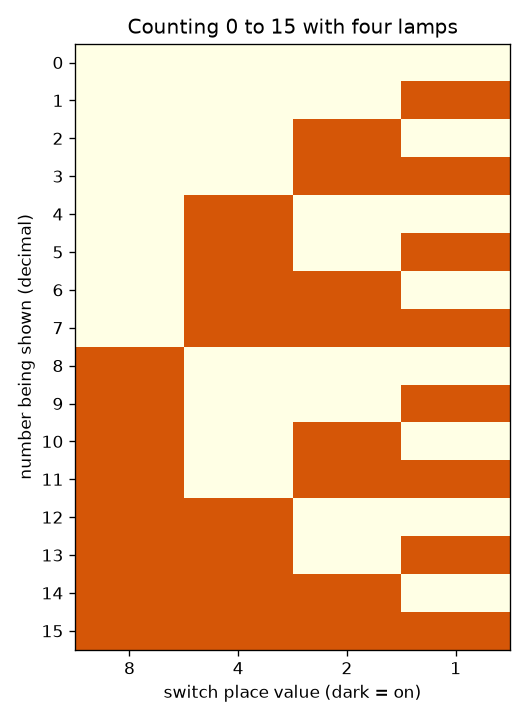
\includegraphics[width=0.85\linewidth]{figures/s01_counting_lamps.png}\\\small Counting 0 to 15: one row per number, dark squares are lamps that are on.\end{center}

\subsection*{E. Worked example}
What number do the switches 1101 show? Then show the number 12 as switches.
\begin{enumerate}[nosep]
\item Write the place values over the switches: 8, 4, 2, 1.
\item Switches on are the first, second and fourth, so add 8 + 4 + 1 and add 0 for the third: 8 + 4 + 0 + 1 = 13.
\item For 12 take the biggest place value that fits: 8 fits (12 - 8 = 4), 4 fits (4 - 4 = 0), 2 and 1 do not.
\item So 12 is 8 + 4 = 1100 (first and second switch on).
\item Check: 8 + 4 + 0 + 0 = 12.
\end{enumerate}
\textbf{Answer.} 1101 shows 13, and 12 is written 1100.

\subsection*{F. Questions}
\begin{enumerate}[nosep]
\item \textbf{Conceptual.} Why does adding one more switch exactly double the number of different patterns?
\item \textbf{Numerical.} Read the switches 1011 as a decimal number, and write 12 as switches. Sanity check each result.
\item \textbf{Graph and simulation interpretation.} In the graph of lamps on against the number, how many numbers between 0 and 15 have exactly two lamps on? What is the highest point of the graph and where does it occur?
\item \textbf{Design and optimisation challenge.} Design: a hall has 100 seats numbered from 0 to 99. A sign should show the seat number on lamps. What is the smallest number of lamps? Name one trade-off of using more lamps than that.
\end{enumerate}

\section{Session 2: Number systems, logic gates and Boolean algebra}

\subsection*{A. Real-world problem}
A stairwell light has a switch at the top and one at the bottom, and either one must toggle the light. A lift must not move unless the door is closed AND the load is within the limit. Rules like these are built from logic gates, tiny circuits whose output is 0 or 1 and depends only on their inputs. To talk about the numbers inside such machines, engineers also write them in hexadecimal, which is binary in a short form. This is a simplified educational model: ideal gates with no electrical detail.

\subsection*{B. Concept and theory}
In base b the digit string d\_k ... d\_1 d\_0 means d\_k b\textasciicircum{}k + ... + d\_1 b + d\_0. To convert a number to base b, divide by b again and again and collect the remainders, last remainder first. Hexadecimal (base 16) uses digits 0 to 9 and A to F (A is 10, F is 15), and each hex digit stands for exactly four bits, so 1011 0111 is B7. A logic gate maps input bits to an output bit. AND gives 1 only if both inputs are 1; OR gives 1 if at least one is 1; NOT flips a bit; XOR gives 1 if the inputs differ; NAND is NOT of AND. A truth table lists the output for every input row, and a claim that is true on every row is proved. De Morgan's laws turn an AND into an OR by flipping inputs and output. Because NAND(a, a) is NOT a, NAND can build NOT, then AND, then OR, then XOR: it is called universal. Any truth table can be turned into a circuit: write one AND term (a minterm) for each row whose output is 1 and OR the terms together (sum of products).

\begin{itemize}[nosep]
\item b: the base of a number system (2, 10 or 16) (no unit)
\item d\_k: digit in place k (no unit)
\item a, b: input bits of a gate (0 or 1)
\item NOT a: the opposite bit of a (written with a bar in equations) (0 or 1)
\item minterm: an AND term that is 1 on exactly one input row (0 or 1)
\end{itemize}

\begin{equation*}
N=\sum_k d_k\,b^{k}
\end{equation*}

\begin{equation*}
\overline{a\cdot b}=\bar a+\bar b,\qquad \overline{a+b}=\bar a\cdot\bar b
\end{equation*}

\begin{equation*}
\bar a=\overline{a\cdot a},\qquad a\cdot b=\overline{\overline{a\cdot b}},\qquad a+b=\overline{\bar a\cdot\bar b}
\end{equation*}

\begin{equation*}
a\oplus b=a\bar b+\bar a b
\end{equation*}

\begin{equation*}
\text{majority}(a,b,c)=\bar a bc+a\bar b c+ab\bar c+abc=ab+ac+bc
\end{equation*}

\begin{center}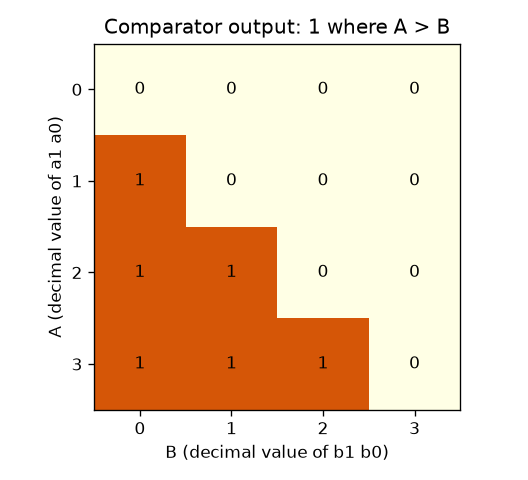
\includegraphics[width=0.85\linewidth]{figures/s02_comparator.png}\\\small The 2-bit comparator: dark where A is greater than B.\end{center}

\subsection*{E. Worked example}
Convert 183 to binary and to hexadecimal, and check by converting back.
\begin{enumerate}[nosep]
\item Divide by 2 repeatedly and collect remainders from last to first. 183 = 128 + 32 + 16 + 4 + 2 + 1, so the bits are 1 0 1 1 0 1 1 1.
\item So 183 is 10110111 in binary.
\item Group in fours from the right: 1011 and 0111. 1011 is 11, which is B, and 0111 is 7.
\item So 183 is B7 in hexadecimal.
\item Check: B7 = 11 x 16 + 7 = 176 + 7 = 183. The same number.
\end{enumerate}
\textbf{Answer.} 183 is 10110111 in binary and B7 in hexadecimal.

\subsection*{F. Questions}
\begin{enumerate}[nosep]
\item \textbf{Conceptual.} Why can NAND build every other gate? Show how to get NOT and OR from NAND.
\item \textbf{Numerical.} Convert the hexadecimal number A5 to decimal and to binary, and convert decimal 100 to binary and hexadecimal. Sanity check.
\item \textbf{Graph and simulation interpretation.} In the comparator figure (A down the side, B along the top, dark where A \textgreater{} B), where are the dark squares and how many are there? Why is the diagonal white?
\item \textbf{Design and optimisation challenge.} Design: a lock opens when the 2-bit number A equals the 2-bit number B. Build the truth table, write the sum-of-products form and give a shorter form with XNOR. How many minterms are there?
\end{enumerate}

\section{Session 3: Build an adder from gates and see how computers count}

\subsection*{A. Real-world problem}
Inside a processor there is no plus button, only gates. Yet it adds very many numbers every second, subtracts, and knows when an answer does not fit. How can a handful of AND, OR and XOR gates add two numbers, and why does it take longer to add 32 bits than 4? We build the arithmetic of a computer from scratch in a tiny simulator and test every circuit against Python's own integers on every possible input. This is a simplified educational model: ideal gates, each with one unit of delay, no clock and no real chip timing.

\subsection*{B. Concept and theory}
A half adder adds two bits: the sum bit is a XOR b (1 when the inputs differ) and the carry bit is a AND b (1 when both are 1). A full adder also takes a carry in: sum = a XOR b XOR c\_in and carry out = ab + (a XOR b) c\_in; it is two half adders and an OR gate, five gates in all. Chain n full adders with the carry out of each feeding the next and you get an n-bit ripple-carry adder. In n-bit two's complement the leftmost bit counts as -2\textasciicircum{}(n-1) instead of +2\textasciicircum{}(n-1), so four bits cover -8 to 7 and 1111 means -1. To negate a number flip every bit and add 1, so a - b = a + (NOT b) + 1: XOR every b bit with a control bit \texttt{sub} and use \texttt{sub} as the carry in, and one adder both adds and subtracts. If the true answer is outside the range, the result wraps round and overflow occurs; it is detected when the carry into the top bit differs from the carry out of it. Each gate takes one unit of delay, and a wire's depth is one more than the depth of its slowest input. The carry out of stage i must wait for the carry out of stage i - 1, so the delay of the last carry grows in a straight line with the width. That is why fast processors use carry-lookahead circuits (a stretch topic) that work out carries in parallel. An ALU (arithmetic logic unit) feeds the same inputs to several operations and a control code selects which result comes out.

\begin{itemize}[nosep]
\item a, b: input bits (or n-bit numbers) (0 or 1)
\item c\_in, c\_out: carry into and out of a stage (0 or 1)
\item n: adder width (bits)
\item sub: control bit: 0 add, 1 subtract (0 or 1)
\item T(n): delay of the last carry out (gate delays)
\item op: ALU control code: 00 add, 01 subtract, 10 AND, 11 OR (2 bits)
\end{itemize}

\begin{equation*}
s=a\oplus b\oplus c_{in},\qquad c_{out}=ab+(a\oplus b)\,c_{in}
\end{equation*}

\begin{equation*}
\text{value}=-b_{n-1}2^{\,n-1}+\sum_{k=0}^{n-2}b_k 2^{k},\qquad -2^{n-1}\le \text{value}\le 2^{n-1}-1
\end{equation*}

\begin{equation*}
a-b=a+\bar b+1\pmod{2^{n}}
\end{equation*}

\begin{equation*}
\text{overflow}=c_{n-1}\oplus c_{n}
\end{equation*}

\begin{equation*}
T(n)=2n+1\ \text{gate delays}
\end{equation*}

\begin{center}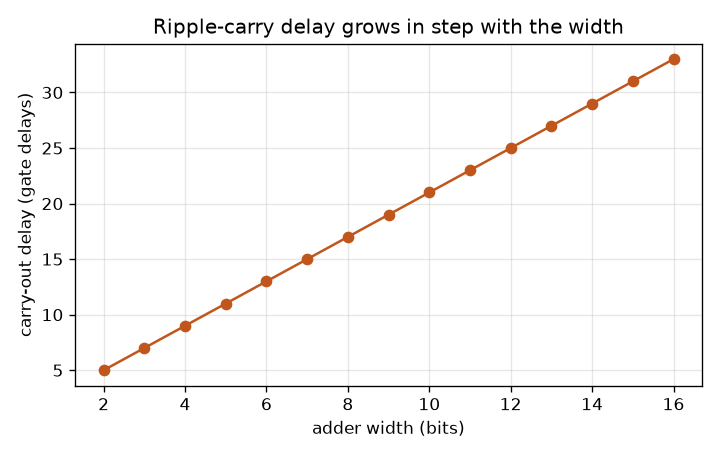
\includegraphics[width=0.85\linewidth]{figures/s03_carry_delay.png}\\\small Carry-out delay of the ripple adder grows in a straight line with its width.\end{center}

\subsection*{E. Worked example}
Compute 6 - 3 on four bits with the adder-subtractor, showing the bits.
\begin{enumerate}[nosep]
\item Subtraction means sub = 1: flip every bit of b and add 1 through the carry in.
\item 6 is 0110 and 3 is 0011; flipping the bits of 3 gives 1100.
\item Add 0110 + 1100 + 1 (the carry in) = 10011.
\item Keep only four bits: 0011, the carry out of the top bit is thrown away.
\item 0011 is 3, and 6 - 3 = 3. The carry into the top bit and the carry out of it are equal, so there is no overflow.
\end{enumerate}
\textbf{Answer.} 6 - 3 = 3, pattern 0011, overflow flag 0.

\subsection*{F. Questions}
\begin{enumerate}[nosep]
\item \textbf{Conceptual.} Why does 7 + 1 give -8 on four bits, and how does the circuit know that the answer is wrong?
\item \textbf{Numerical.} Compute 5 - 7 on four bits: show the three numbers you add, the four-bit result, and whether overflow occurs. Sanity check with ordinary arithmetic.
\item \textbf{Graph and simulation interpretation.} From the delay graph, how many gate delays does the carry take for 8 bits, and for 12 bits? What does the slope of the line tell you?
\item \textbf{Design and optimisation challenge.} Design: each gate takes 0.5 ns and the carry out of a ripple adder must be ready within 20 ns. What is the widest adder allowed? What would you change to go wider?
\end{enumerate}

\section{Real-world mini-project}
\textbf{Build and test an 8-bit adder-subtractor.} A small calculator chip needs to add and subtract 8-bit numbers (-128 to 127) and to warn when the answer does not fit. Use \texttt{build\_add\_sub(8)} and \texttt{add\_sub} from Session 3. Test it on every pair of inputs for both operations against Python integers, count the pairs that overflow, count its gates, read the delay of its overflow flag, and then decide the widest adder-subtractor whose overflow flag is ready within a 10 ns budget if one gate takes 0.5 ns.

\section{The path ahead}
\begin{enumerate}[nosep]
\item \textbf{Session 4: A carry-lookahead adder.} A 16-bit adder built in the simulator whose carries do not ripple.
\item \textbf{Session 5: A 4-bit multiplier.} A 4 x 4 multiplier made of gates with an 8-bit product.
\item \textbf{Session 6: A saturating adder.} An 8-bit adder-subtractor that returns the nearest extreme on overflow.
\item \textbf{Session 7: A counter that remembers.} A 4-bit counter driven by clock ticks.
\item \textbf{Session 8: An ALU with flags and a decoder.} An 8-bit ALU with four operations and flags, and a decoder lighting the right segments for each digit.
\end{enumerate}

\section{Answers and hints}

\subsection*{Session 1}
\begin{enumerate}[nosep]
\item \textbf{Conceptual.} Hint: Take every pattern you already had and ask how many ways the new switch can be set. Solution: Each old pattern can be combined with the new switch off or on, which gives two new patterns for every old one. Four switches make 16 patterns, five make 32. So n switches make 2\textasciicircum{}n patterns, and the largest number is 2\textasciicircum{}n - 1 because the counting starts at 0.
\item \textbf{Numerical.} Hint: Use the place values 8, 4, 2, 1. Solution: 1011 = 8 + 0 + 2 + 1 = 11. For 12: 8 + 4 = 12, so the pattern is 1100. Sanity check: 11 is below 15 (the largest on 4 switches) and 1100 sums back to 12.
\item \textbf{Graph and simulation interpretation.} Hint: Count the dots at height 2, and look for the number with every switch on. Solution: Six numbers have exactly two lamps on: 3, 5, 6, 9, 10 and 12. The graph is highest (4 lamps) at 15, where every switch is on, and lowest (0 lamps) at 0. The counts at heights 0 to 4 are 1, 4, 6, 4, 1.
\item \textbf{Design and optimisation challenge.} Hint: Find the smallest n with 2\textasciicircum{}n at least 100. Solution: 6 lamps give only 64 patterns, which is not enough. 7 lamps give 128 patterns, which covers 0 to 99, so 7 lamps are enough and 7 is the smallest number. Using 8 or more lamps would cost more parts and more wiring while only wasting patterns; using fewer is impossible. Assumption: one lamp per bit and a fixed, known maximum seat number.
\end{enumerate}

\subsection*{Session 2}
\begin{enumerate}[nosep]
\item \textbf{Conceptual.} Hint: What does NAND do when both inputs are the same wire? Then use De Morgan. Solution: NAND(a, a) is NOT(a AND a) = NOT a, so NAND gives NOT. AND is NOT of NAND, so AND takes two NAND gates. OR(a, b) = NOT(NOT a AND NOT b) = NAND(NOT a, NOT b), which takes three NAND gates. XOR takes four. With NOT and AND you can build any truth table, so NAND alone is enough.
\item \textbf{Numerical.} Hint: A is 10. Each hex digit is four bits. Solution: A5 = 10 x 16 + 5 = 165, and A = 1010, 5 = 0101, so A5 is 10100101. For 100: 64 + 32 + 4 = 100, so it is 1100100 in binary; grouping 0110 0100 gives 64 in hexadecimal (6 x 16 + 4 = 100). Check: 10100101 = 128 + 32 + 4 + 1 = 165.
\item \textbf{Graph and simulation interpretation.} Hint: On the diagonal A and B are equal. Solution: There are six dark squares, all below the diagonal (the row number A is larger than the column number B): 3 + 2 + 1 = 6. The diagonal is white because there A = B, so A \textgreater{} B is false. The squares above the diagonal are white because there B is larger.
\item \textbf{Design and optimisation challenge.} Hint: List the 16 rows (a1 a0 b1 b0) and mark those with A = B. XNOR is 1 when its inputs are the same. Solution: A = B on four rows: 0000, 0101, 1010, 1111, so there are 4 minterms out of 16. Sum of products: the OR of those four 4-input AND terms. Shorter: (a1 XNOR b1) AND (a0 XNOR b0), because A = B exactly when each bit pair matches. Trade-off: the sum of products is mechanical and always works, the short form uses fewer gates but needs insight. We checked both on all 16 rows.
\end{enumerate}

\subsection*{Session 3}
\begin{enumerate}[nosep]
\item \textbf{Conceptual.} Hint: Write 0111 + 0001, and compare the carry into the top bit with the carry out of it. Solution: 0111 + 0001 = 1000. Read as two's complement, 1000 is -8, because the top bit has the weight -8. The true answer 8 does not fit in -8 to 7, so the result wrapped round. The carry into the top bit is 1 but the carry out of it is 0; they differ, so the overflow flag is 1.
\item \textbf{Numerical.} Hint: Flip the bits of 7 (0111), add 0101 and add the carry in 1. Solution: NOT 0111 = 1000. Add 0101 + 1000 + 1 = 1110 (14). Read as two's complement, 1110 is 14 - 16 = -2. Check: 5 - 7 = -2, and -2 is inside -8 to 7, so overflow is 0.
\item \textbf{Graph and simulation interpretation.} Hint: The line is T(n) = 2n + 1. Solution: For 8 bits T = 17 gate delays; for 12 bits T = 2 x 12 + 1 = 25. The slope is 2 gate delays per extra bit, the two gates (AND then OR) that the carry passes through in every stage. Doubling the width roughly doubles the delay, which is the reason for carry-lookahead.
\item \textbf{Design and optimisation challenge.} Hint: Solve (2n + 1) x 0.5 \textless{}= 20. Solution: (2n + 1) x 0.5 \textless{}= 20 gives 2n + 1 \textless{}= 40, so n \textless{}= 19.5 and the widest is 19 bits (39 gate delays = 19.5 ns; 20 bits would need 41 gate delays = 20.5 ns). To go wider, use a carry-lookahead adder, or split the work over two clock cycles. Trade-off: lookahead needs more gates for less delay.
\end{enumerate}

\section{How to join}
Read \texttt{CONTRIBUTING.md} in the repository, then pick an issue labelled \texttt{good first issue}. Repository: \url{https://github.com/KrunalPanchal1995/openbinary}

\end{document}
